\documentclass[journal,12pt,twocolumn]{IEEEtran}
%

\def\inputGnumericTable{}
\usepackage{setspace}
\usepackage{gensymb}
%\doublespacing
\singlespacing

%\usepackage{graphicx}
%\usepackage{amssymb}
%\usepackage{relsize}
\usepackage[cmex10]{amsmath}
%\usepackage{amsthm}
%\interdisplaylinepenalty=2500
%\savesymbol{iint}
%\usepackage{txfonts}
%\restoresymbol{TXF}{iint}
%\usepackage{wasysym}
\usepackage{amsthm}
%\usepackage{iithtlc}
\usepackage{mathrsfs}
\usepackage{txfonts}
\usepackage{stfloats}
\usepackage{bm}
\usepackage{cite}
\usepackage{cases}
\usepackage{subfig}
%\usepackage{xtab}
\usepackage{longtable}
\usepackage{multirow}
%\usepackage{algorithm}
%\usepackage{algpseudocode}
\usepackage{enumitem}
\usepackage{mathtools}
\usepackage{steinmetz}
\usepackage{tikz}
\usepackage{circuitikz}
\usepackage{verbatim}
\usepackage{tfrupee}
\usepackage[breaklinks=true]{hyperref}
%\usepackage{stmaryrd}
\usepackage{tkz-euclide} % loads  TikZ and tkz-base
%\usetkzobj{all}
\usetikzlibrary{calc,math}
\usepackage{listings}
    \usepackage{color}                                            %%
    \usepackage{array}                                            %%
    \usepackage{longtable}                                        %%
    \usepackage{calc}                                             %%
    \usepackage{multirow}                                         %%
    \usepackage{hhline}                                           %%
    \usepackage{ifthen}                                           %%
  %optionally (for landscape tables embedded in another document): %%
    \usepackage{lscape}     
\usepackage{multicol}
\usepackage{chngcntr}
%\usepackage{enumerate}

%\usepackage{wasysym}
%\newcounter{MYtempeqncnt}
\DeclareMathOperator*{\Res}{Res}
%\renewcommand{\baselinestretch}{2}
\renewcommand\thesection{\arabic{section}}
\renewcommand\thesubsection{\thesection.\arabic{subsection}}
\renewcommand\thesubsubsection{\thesubsection.\arabic{subsubsection}}

\renewcommand\thesectiondis{\arabic{section}}
\renewcommand\thesubsectiondis{\thesectiondis.\arabic{subsection}}
\renewcommand\thesubsubsectiondis{\thesubsectiondis.\arabic{subsubsection}}

% correct bad hyphenation here
\hyphenation{op-tical net-works semi-conduc-tor}
\def\inputGnumericTable{}                                 %%

\lstset{
%language=C,
frame=single, 
breaklines=true,
columns=fullflexible
}
%\lstset{
%language=tex,
%frame=single, 
%breaklines=true
%}

\begin{document}
%


\newtheorem{theorem}{Theorem}[section]
\newtheorem{problem}{Problem}
\newtheorem{proposition}{Proposition}[section]
\newtheorem{lemma}{Lemma}[section]
\newtheorem{corollary}[theorem]{Corollary}
\newtheorem{example}{Example}[section]
\newtheorem{definition}[problem]{Definition}
%\newtheorem{thm}{Theorem}[section] 
%\newtheorem{defn}[thm]{Definition}
%\newtheorem{algorithm}{Algorithm}[section]
%\newtheorem{cor}{Corollary}
\newcommand{\BEQA}{\begin{eqnarray}}
\newcommand{\EEQA}{\end{eqnarray}}
\newcommand{\define}{\stackrel{\triangle}{=}}
\bibliographystyle{IEEEtran}
%\bibliographystyle{ieeetr}
\providecommand{\mbf}{\mathbf}
\providecommand{\pr}[1]{\ensuremath{\Pr\left(#1\right)}}
\providecommand{\qfunc}[1]{\ensuremath{Q\left(#1\right)}}
\providecommand{\sbrak}[1]{\ensuremath{{}\left[#1\right]}}
\providecommand{\lsbrak}[1]{\ensuremath{{}\left[#1\right.}}
\providecommand{\rsbrak}[1]{\ensuremath{{}\left.#1\right]}}
\providecommand{\brak}[1]{\ensuremath{\left(#1\right)}}
\providecommand{\lbrak}[1]{\ensuremath{\left(#1\right.}}
\providecommand{\rbrak}[1]{\ensuremath{\left.#1\right)}}
\providecommand{\cbrak}[1]{\ensuremath{\left\{#1\right\}}}
\providecommand{\lcbrak}[1]{\ensuremath{\left\{#1\right.}}
\providecommand{\rcbrak}[1]{\ensuremath{\left.#1\right\}}}
\theoremstyle{remark}
\newtheorem{rem}{Remark}
\newcommand{\sgn}{\mathop{\mathrm{sgn}}}
\providecommand{\abs}[1]{\left\vert#1\right\vert}
\providecommand{\res}[1]{\Res\displaylimits_{#1}} 
\providecommand{\norm}[1]{\left\lVert#1\right\rVert}
%\providecommand{\norm}[1]{\lVert#1\rVert}
\providecommand{\mtx}[1]{\mathbf{#1}}
\providecommand{\mean}[1]{E\left[ #1 \right]}
\providecommand{\fourier}{\overset{\mathcal{F}}{ \rightleftharpoons}}
%\providecommand{\hilbert}{\overset{\mathcal{H}}{ \rightleftharpoons}}
\providecommand{\system}{\overset{\mathcal{H}}{ \longleftrightarrow}}
	%\newcommand{\solution}[2]{\textbf{Solution:}{#1}}
\newcommand{\solution}{\noindent \textbf{Solution: }}
\newcommand{\cosec}{\,\text{cosec}\,}
\providecommand{\dec}[2]{\ensuremath{\overset{#1}{\underset{#2}{\gtrless}}}}
\newcommand{\myvec}[1]{\ensuremath{\begin{pmatrix}#1\end{pmatrix}}}
%\newcommand{\myvec}[1]{\ensuremath{\begin{pmatrix}#1\end{pmatrix}}}
\newcommand{\mydet}[1]{\ensuremath{\begin{vmatrix}#1\end{vmatrix}}}
%\numberwithin{equation}{section}
\numberwithin{equation}{subsection}
%\numberwithin{problem}{section}
%\numberwithin{definition}{section}
\makeatletter
\@addtoreset{figure}{problem}
\makeatother
\let\StandardTheFigure\thefigure
\let\vec\mathbf
%\renewcommand{\thefigure}{\theproblem.\arabic{figure}}
%\renewcommand{\thefigure}{\theproblem}
%\setlist[enumerate,1]{before=\renewcommand\theequation{\theenumi.\arabic{equation}}
%\counterwithin{equation}{enumi}
%\renewcommand{\theequation}{\arabic{subsection}.\arabic{equation}}
\def\putbox#1#2#3{\makebox[0in][l]{\makebox[#1][l]{}\raisebox{\baselineskip}[0in][0in]{\raisebox{#2}[0in][0in]{#3}}}}
     \def\rightbox#1{\makebox[0in][r]{#1}}
     \def\centbox#1{\makebox[0in]{#1}}
     \def\topbox#1{\raisebox{-\baselineskip}[0in][0in]{#1}}
     \def\midbox#1{\raisebox{-0.5\baselineskip}[0in][0in]{#1}}
\vspace{3cm}
\title{LinearAlgebra Question 5}
\author{Srihari S}


\maketitle
\begin{abstract}
A document implementing solutions to problems using linear algebra.
\end{abstract}
Download all python codes from 
%
\begin{lstlisting}
svn co https://github.com/Srihari123456/Summer-2020/tree/master/LinearAlgebrafolder/codes
\end{lstlisting}
Download all \LaTeX{}-Tikz codes from 
%
\begin{lstlisting}
svn co https://github.com/Srihari123456/Summer-2020/tree/master/LinearAlgebrafolder/figs
\end{lstlisting}

%\section{\textbf{Question 1.1.5}}
%\subsection{Problem}
\renewcommand{\theequation}{\theenumi}
\begin{enumerate}[label=\thesection.\arabic*.,ref=\thesection.\theenumi]
\numberwithin{equation}{enumi}
\item Find the area of the triangle having vertices 
\begin{multline}
	\vec{A} = \myvec{1\\1\\1}\quad
	\vec{B} = \myvec{1\\2\\3}\quad
	\vec{C} = \myvec{2\\3\\1}
\end{multline}
	The following python code computes the area of $\triangle$ABC in Fig.\ref{fig:qone}.
	\begin{lstlisting}
	./codes/triangle/q1.py
	\end{lstlisting}
	\solution The area of $\triangle$ABC is defined as
	\begin{align}
		\frac{1}{2}\norm{\brak{\vec{B-A}} \times \brak{\vec{C-A}}}
	\end{align}
	\begin{figure}[!ht]
	\centering
	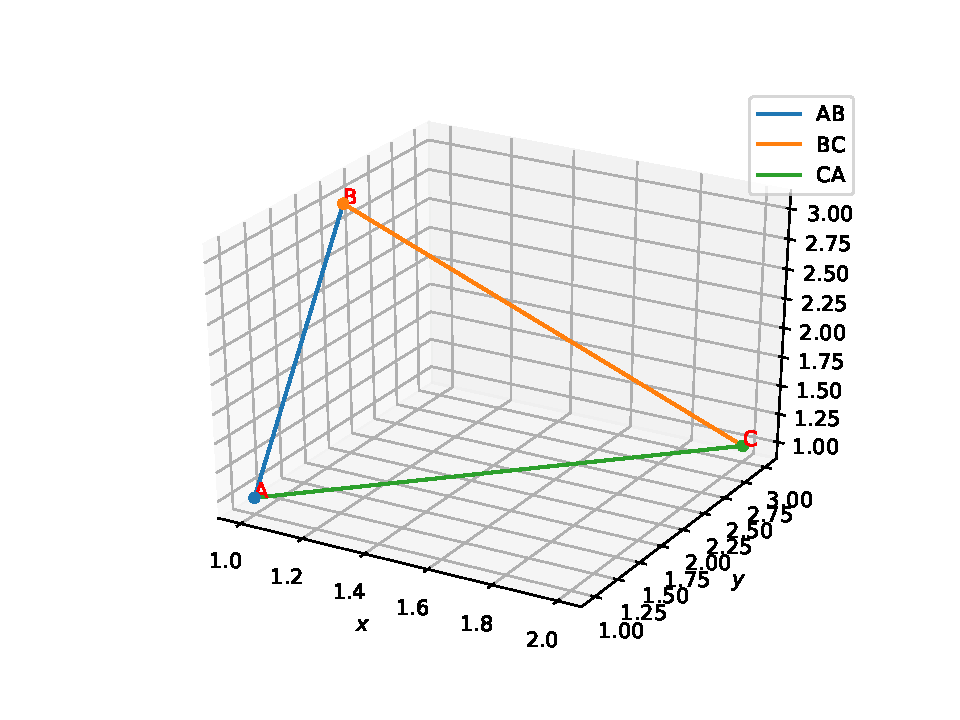
\includegraphics[width=\columnwidth]{./figs/triangle/q1.pdf}
	\caption{Triangle of Q.1.1.5}
	\label{fig:qone}	
	\end{figure}
	which is calculated and found as 2.29
\end{enumerate}


\section{\textbf{Question 1.2.5}}
\subsection{Problem}
\renewcommand{\theequation}{\theenumi}
\begin{enumerate}[label=\thesection.\arabic*.,ref=\thesection.\theenumi]
\numberwithin{equation}{enumi}

\item In $\triangle$ABC with vertices 
\begin{multline}
\vec{A} = \myvec{2\\3}\quad
\vec{B} = \myvec{4\\-1}\quad
\vec{C} = \myvec{1\\2}
\end{multline}
	Find the equation and the length of the altitude from vertex $\vec{A}$.
	The following python code computes the length of the altitude $\vec{AD}$ in Fig.\ref{fig:qtwo}.
	\begin{lstlisting}
	./codes/triangle/q2.py
	\end{lstlisting}
	
	\begin{figure}[!ht]
	\centering
	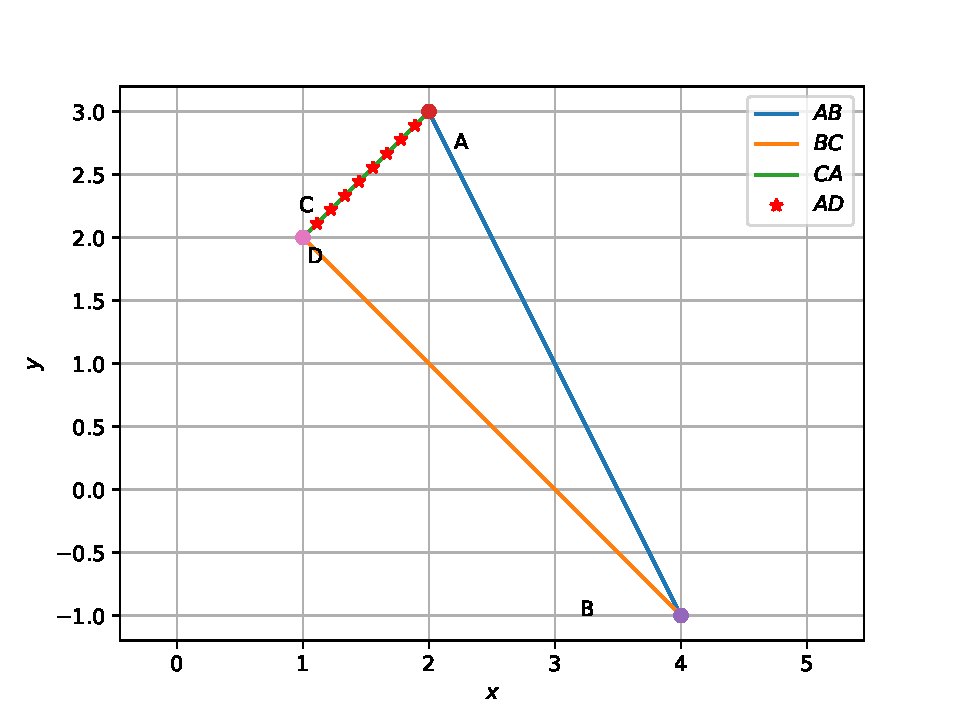
\includegraphics[width=\columnwidth]{./figs/triangle/q2.pdf}
	\caption{Triangle of Q.1.2.5}
	\label{fig:qtwo}	
	\end{figure}
	
	
	\solution 
	\begin{multline}
	\because \norm{\vec{B-A}}^2 = \norm{\vec{B-C}}^2 + \norm{\vec{C-A}}^2\\
	\triangle \text{ ABC is right angled.}
	\end{multline}
	
	Let the direction vector $\vec{m = B-C}$
	We define the normal vector
	\begin{align}
		\vec{n} = \myvec{0&1\\-1&0}\vec{m}
	\end{align}
	Equation of line $\vec{AD}$ is obtained as:
	\begin{align}
		\vec{m^Tx} &= \vec{m^TA}
		\\
		\myvec{3&-3}\vec{x} &= -3
	\end{align}
	
	Equation of line $\vec{BC}$ is :
	\begin{align}
		\vec{n^Tx} = \vec{n^TB}
	\end{align}
	
	Since $\vec{D}$ is the intersection of lines $\vec{AD}$ and $\vec{BC}$ 
	\begin{multline}
		\myvec{\vec{m}&\vec{n}}^T \vec{D}= \myvec{\vec{m^TA}\\\vec{n^TB}}
		\\
	\text{which is solved to obtain the value of }\vec{D} = \myvec{1\\2}
	\end{multline}
	
	Therefore  The length of the altitude is obtained as $\norm{\vec{A-D}} = 1.414$
	
	
	
	
\end{enumerate}

%\section{\textbf{Question 2.1.5}}
%\subsection{Problem}
\renewcommand{\theequation}{\theenumi}
\begin{enumerate}[label=\thesection.\arabic*.,ref=\thesection.\theenumi]
\numberwithin{equation}{enumi}

\item Find the area of a parallelogram whose adjacent sides are given by the vectors 
	$\myvec{3\\1\\4}$ and $\myvec{1\\-1\\1}$\\
	The following python code computes the area of required parallelogram.
	\begin{lstlisting}
	./codes/quadrilateral/q3.py
	\end{lstlisting}
	
	\solution The area is given as
	\begin{align}
	\frac{1}{2}\norm{\myvec{3\\1\\4}\times\myvec{1\\-1\\1}}
	\end{align}
	which is calculated and found as 3.24
\end{enumerate}

\section{\textbf{Question 2.2.5}}
\subsection{Problem}

\renewcommand{\theequation}{\theenumi}
\begin{enumerate}[label=\thesection.\arabic*.,ref=\thesection.\theenumi]
\numberwithin{equation}{enumi}
	\item Without using distance formula, show that the points
	\begin{multline}
	\vec{A} = \myvec{-2\\-1} \quad \vec{B} = \myvec{4\\0} \quad \vec{C} = \myvec{3\\3}\text{ and }\vec{D} = \myvec{-3\\2} 
	\end{multline}
	are the vertices of a parallelogram.
The following python code computes the area of $\triangle$ABC in Fig.\ref{fig:qfour}.
	\begin{lstlisting}
	./codes/quadrilateral/q4.py
	\end{lstlisting}
	
	\solution As the direction vectors,
	\begin{align}
	\vec{A - B}=\vec{D - C}
	\\
	\vec{A - D}=\vec{B - C}
	\end{align}
	
	\begin{figure}[!ht]
	\centering
	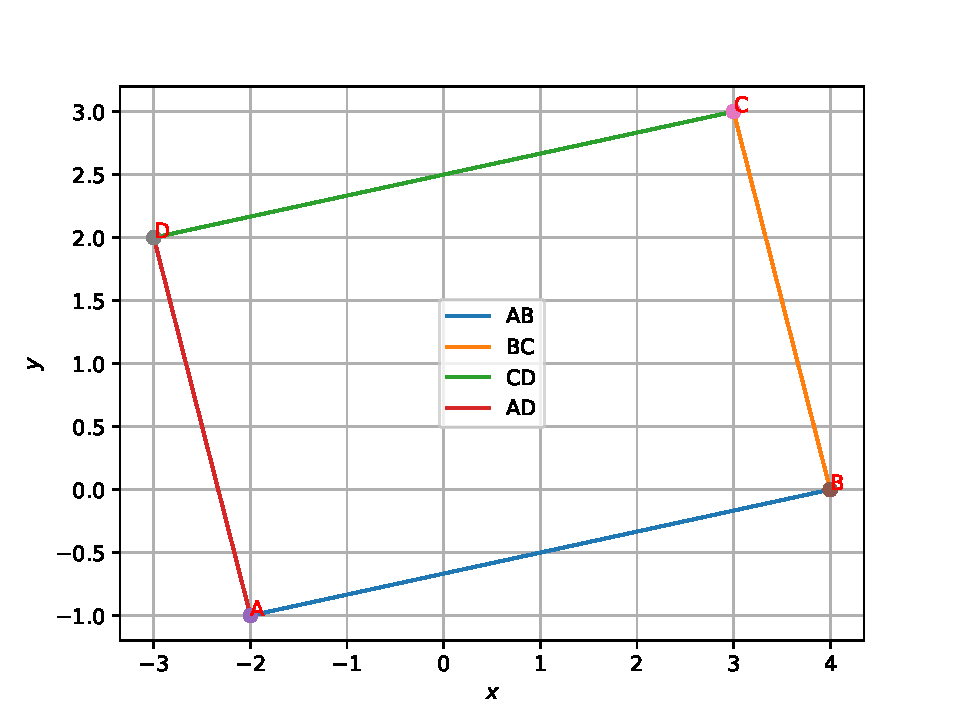
\includegraphics[width=\columnwidth]{./figs/quadrilateral/q4.pdf}
	\caption{Parallelogram of Q.2.2.5}
	\label{fig:qfour}	
	\end{figure}
	
	\begin{multline}
	\implies \vec{AB} \parallel \vec{CD}\text{ and }\vec{AD} \parallel \vec{BC}
	\\
	\therefore \vec{ABCD}\text{ is a parallelogram.}
	\end{multline}
\end{enumerate}

%\section{\textbf{Question 3.1.5}}
%\subsection{Problem}

\renewcommand{\theequation}{\theenumi}
\begin{enumerate}[label=\thesection.\arabic*.,ref=\thesection.\theenumi]
\numberwithin{equation}{enumi}
	\item Two rails are represented as 
	\begin{multline}
	\myvec{1&2}\vec{x}=4\text{ and }\myvec{2&4}\vec{x}=12.
	\end{multline}
	\quad Will the rails cross each other?
	
	\solution The above equations can be represented as a matrix equation as
	\begin{align}\myvec{1&2\\2&4}\vec{x}=\myvec{4\\12}\vec{x}\end{align}
	The augmented matrix for the above matrix is row reduced as follows:
	\begin{align}\myvec{1&2&4\\2&4&12}\xleftrightarrow {R_2\leftarrow \frac{R_2}{2}}\myvec{1 & 2 & 4\\1 & 2 & 6} \\
\xleftrightarrow {R_2\leftarrow R_2 - R_1}\myvec{1 & 2 & 4\\0 & 0 & 2}
\end{align}
	Thus the row reduction of the 2$\times$3 matrix 
	\begin{align}
		\myvec{1&2&4\\2&4&12}
	\end{align}
	results in a matrix with two non zero rows having rank 2. Similarly the rank is 1 for the matrix$\myvec{1&2\\2&4}$\\
	As the rank of these two matrices aren't same, there is no solution. Therefore, the rails don't cross over eachother.
	The following python code computes the area of $\triangle$ABC in Fig.\ref{fig:qfive}.
	\begin{lstlisting}
	./codes/lines/q5.py
	\end{lstlisting}
	\begin{figure}[!ht]
	\centering
	\includegraphics[width=\columnwidth]{./figs/lines/q5.eps}
	\caption{Rails of Q.3.1.5}
	\label{fig:qfive}	
	\end{figure}
	
\end{enumerate}

\section{\textbf{Question 3.2.5}}
\subsection{Problem}

\renewcommand{\theequation}{\theenumi}
\begin{enumerate}[label=\thesection.\arabic*.,ref=\thesection.\theenumi]
\numberwithin{equation}{enumi}
\item Solve $\vec{x+y}<5$ graphically.
The following python code computes the graphical representation of $\vec{x+y}<5$ as shown in Fig.\ref{fig:qsix}.
	\begin{lstlisting}
	./codes/lines/q6.py
	\end{lstlisting}
	\begin{figure}[!ht]
	\centering
	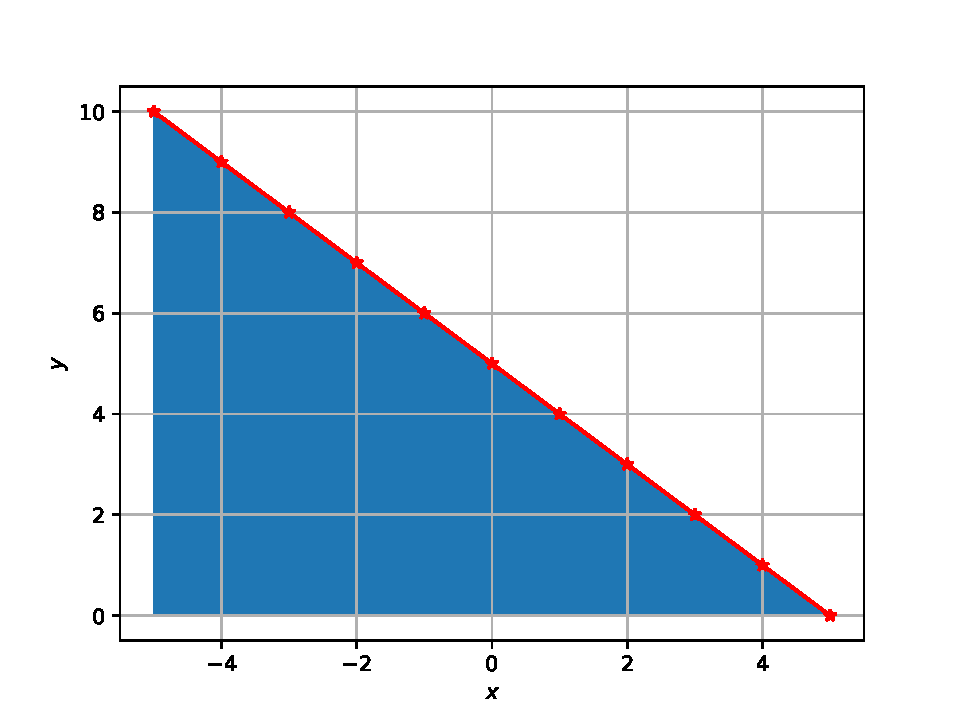
\includegraphics[width=\columnwidth]{./figs/lines/q6.pdf}
	\caption{x+y$<$5}
	\label{fig:qsix}	
	\end{figure}
	
\end{enumerate}

\section{\textbf{Question 3.3.5}}
\subsection{Problem}
\renewcommand{\theequation}{\theenumi}
\begin{enumerate}[label=\thesection.\arabic*.,ref=\thesection.\theenumi]
\numberwithin{equation}{enumi}
\item Find the values of a,b,c,x,y and z if
\begin{multline}
\myvec{x+3&z+4&2y-7\\-6&a-1&0\\b-3&-21&0} = \myvec{0&6&3y-2\\-6&-3&2c+2\\2b+4&-21&0}
\end{multline}
\solution As the two matrices are equal their corresponding entries are also equal. Hence
\begin{align}
x+3=0 \quad \implies x=-3
\\
z+4=6 \quad \implies z=2
\\
2y-7=3y-2 \quad \implies y=-5
\\
a-1=-3 \quad \implies a=-2
\\
2c+2=0 \quad \implies c=-1
\\
b-3=2b+4 \quad \implies b=-7
\end{align}
\end{enumerate}

\section{\textbf{Question 3.5.5}}
\subsection{Problem}

\renewcommand{\theequation}{\theenumi}
\begin{enumerate}[label=\thesection.\arabic*.,ref=\thesection.\theenumi]
\numberwithin{equation}{enumi}
	\item Find the angle between the x-axis and the line joining the points 
	\begin{align}
\vec{A} = \myvec{3\\-1}\text{ and }\vec{B} = \myvec{4\\-2}.
	\end{align}
	The following python code computes the angle which the line in Fig.\ref{fig:qnine} makes with x-axis.
	\begin{lstlisting}
	./codes/lines/q9.py
	\end{lstlisting}
	
	\solution The slope of line $\vec{AB}$ is given as:
	\begin{align}
\tan \theta = \frac{B[1]-A[1]}{B[0]-A[0]}
		\\
\text{which on computing yields} \quad \tan \theta = -1
\\
\therefore \theta = \tan^{-1}(-1) = 135\degree	
	\end{align}

	\begin{figure}[!ht]
	\centering
	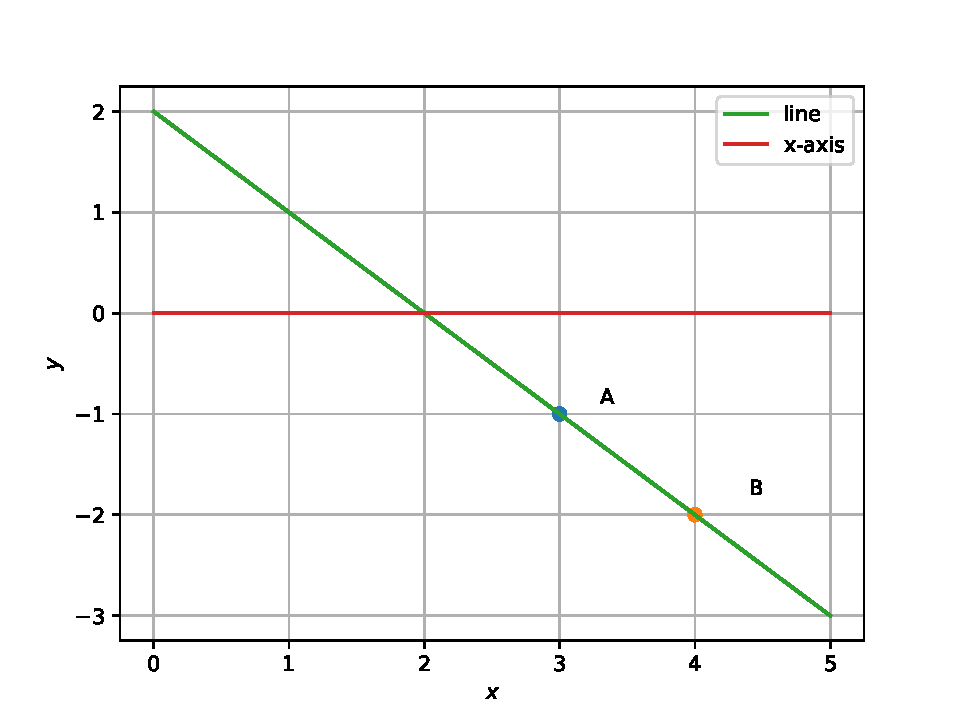
\includegraphics[width=\columnwidth]{./figs/lines/q9.pdf}
	\caption{Line of Q.3.5.5}
	\label{fig:qnine}	
	\end{figure}
	
\end{enumerate}


\section{\textbf{Question 3.6.5}}
\subsection{Problem}

\renewcommand{\theequation}{\theenumi}
\begin{enumerate}[label=\thesection.\arabic*.,ref=\thesection.\theenumi]
\numberwithin{equation}{enumi}
	\item If the vertices of a parallelogram taken in order are
	\begin{multline}
\vec{A}=\myvec{1\\2} , \vec{B}=\myvec{4\\y} ,\vec{C}=\myvec{x\\6}\text{ and }\vec{D}=\myvec{3\\5}\\\text{find x and y.}
\end{multline}
	The following python code computes the value of x and y used in Fig.\ref{fig:qten}.
	\begin{lstlisting}
	./codes/lines/q10.py
	\end{lstlisting}
	
	\solution In a parallelogram, the diagonals bisect each other. Hence
	\begin{align}
		\vec{\frac{A+C}{2} = \frac{B+D}{2}}
		\\
\therefore \vec{\frac{1+x}{2} = \frac{7}{2}}\text{ and }\vec{\frac{8}{2} = \frac{y+5}{2}} \\
\implies x=6,y=3
\end{align}
	\begin{figure}[!ht]
	\centering
	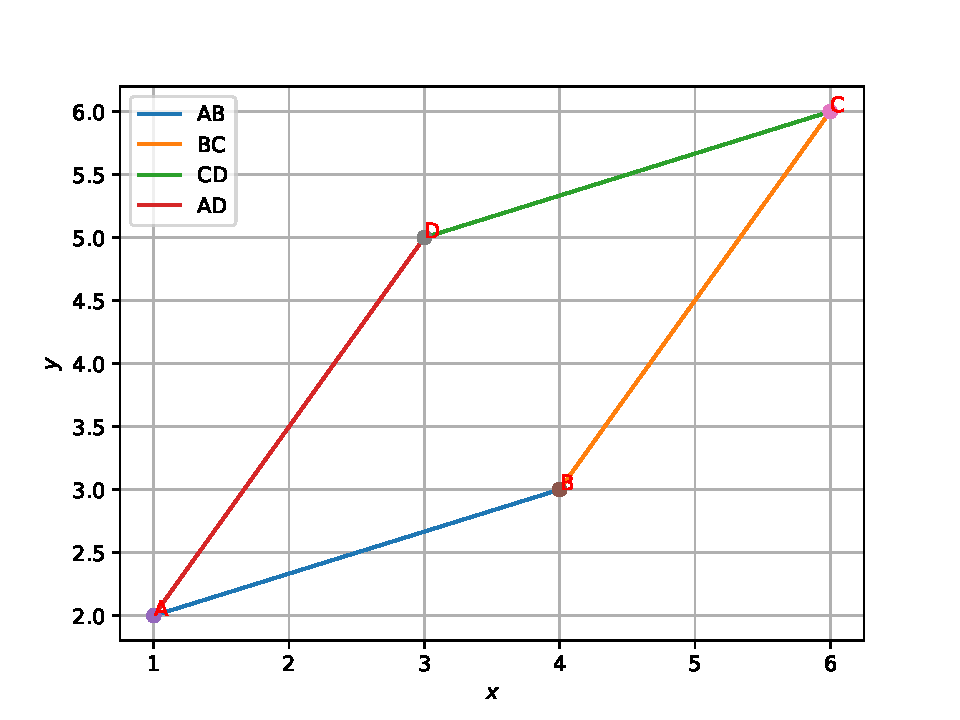
\includegraphics[width=\columnwidth]{./figs/lines/q10.pdf}
	\caption{Parallelogram of Q.3.6.5}
	\label{fig:qten}	
	\end{figure}
	
		
\end{enumerate}

\section{\textbf{Question 3.7.5}}
\subsection{Problem}

\renewcommand{\theequation}{\theenumi}
\begin{enumerate}[label=\thesection.\arabic*.,ref=\thesection.\theenumi]
\numberwithin{equation}{enumi}
	\item Draw the graphs of the following equations:
	\begin{enumerate}
		\item $\myvec{1&1}\vec{x}=0$	
		\item $\myvec{2&-1}\vec{x}=0$
		\item $\myvec{1&-1}\vec{x}=0$
		\item $\myvec{2&-1}\vec{x}=-1$
		\item $\myvec{2&-1}\vec{x}=4$
		\item $\myvec{1&-1}\vec{x}=4$
	\end{enumerate}
	The following python codes draw the graphs which are represented in Fig.\ref{fig:qelevena} and Fig.\ref{fig:qelevenb}.
	\begin{lstlisting}
	./codes/lines/q11a.py
	./codes/lines/q11b.py
	\end{lstlisting}
	\solution
	\begin{figure}[!ht]
	\centering
	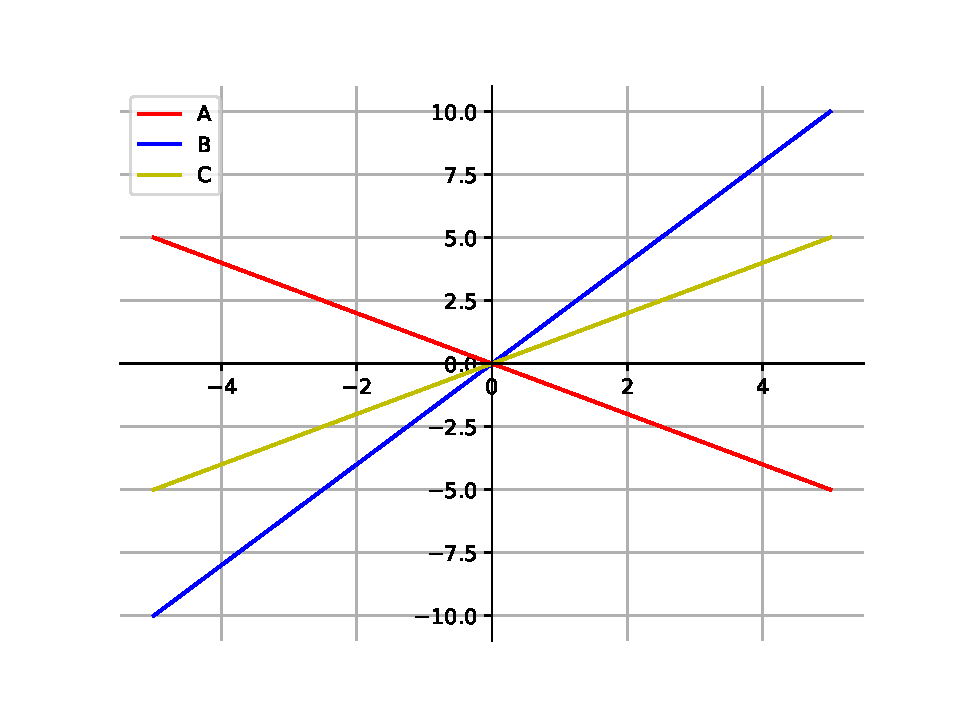
\includegraphics[width=\columnwidth]{./figs/lines/q11a.pdf}
	\caption{Lines of Q.3.7.5}
	\label{fig:qelevena}	
	\end{figure}
	\begin{figure}[!ht]
	\centering
	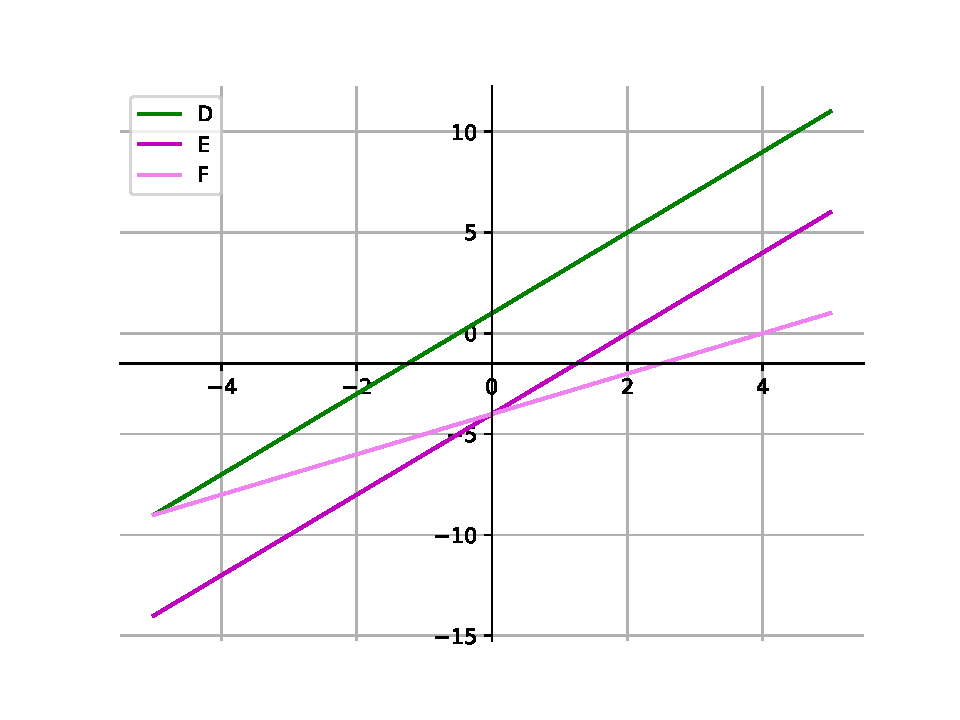
\includegraphics[width=\columnwidth]{./figs/lines/q11b.pdf}
	\caption{Lines of Q.3.7.5}
	\label{fig:qelevenb}	
	\end{figure}
	
\end{enumerate}

\section{\textbf{Question 3.8.5}}
\subsection{Problem}

\renewcommand{\theequation}{\theenumi}
\begin{enumerate}[label=\thesection.\arabic*.,ref=\thesection.\theenumi]
\numberwithin{equation}{enumi}
	\item Rain is falling vertically with a speed of $35ms^{-1}$. A woman rides a bicycle with a speed of $12ms^{-1}$ in east to west direction.What is the direction in which she should hold her umbrella?\\
The following python code computes the area of $\triangle$ABC in Fig.\ref{fig:qtwelve}.
	\begin{lstlisting}
	./codes/lines/q12.py
	\end{lstlisting}
	
	\solution At time t=0 let
\begin{align}
\vec{B} = \myvec{0\\0}
\end{align}
 denote the position of the woman. Since she rides her bicycle at $12ms^{-1}$ in east to west direction , her position at time t=1 is represented as 
\begin{align}
\vec{C} = \myvec{-12\\0}
\end{align}
. Let the position of a rain-droplet at time t=0 be 
\begin{align}
\vec{A} = \myvec{-12\\35}
\end{align}
. The drops which are falling a little ahead of the current position of the woman, will fall on her, because she moves in that direction.
To find the direction in which she should hold her umbrella, we need to find $\angle{CAB} =\theta$. 
\begin{multline}  
	\vec{AB = B-A} = \myvec{12\\-35}
	\\
	\vec{AC = C-A} = \myvec{0\\-35}
	\\
	\vec{AB}^T\vec{AC} = \norm{\vec{AB}}\norm{\vec{AC}}\cos{\theta}
	\\
	\cos{\theta} = \frac{35}{37}
	\\
	\theta = 18.93\degree 
\end{multline}
So the cyclist should hold the umbrella at 18.93$\degree$ to the vertical in the forward direction.

\begin{figure}[!ht]
	\centering
	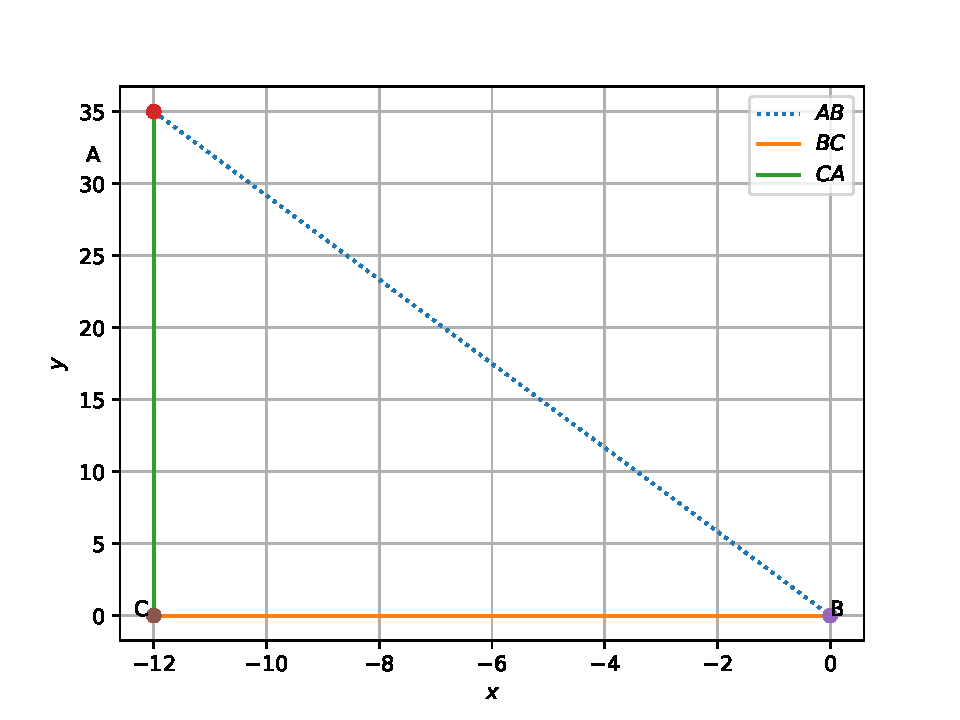
\includegraphics[width=\columnwidth]{./figs/lines/q12.pdf}
	\caption{Figure of Q.3.8.5}
	\label{fig:qtwelve}	
	\end{figure}
	


\end{enumerate}

\section{\textbf{Question 3.9.5}}
\subsection{Problem}

\renewcommand{\theequation}{\theenumi}
\begin{enumerate}[label=\thesection.\arabic*.,ref=\thesection.\theenumi]
\numberwithin{equation}{enumi}
	\item Construct a a3$\times$4 matrix whose elements are given by:
	\begin{enumerate}
		\item $A_{ij} = \frac{1}{2}|-3i+j|$
		\item $A_{ij} = 2i-j$
	\end{enumerate}
	
	The following python code computes the required matrix.
	\begin{lstlisting}
	./codes/lines/q13.py
	\end{lstlisting}
	
	\solution 
	\begin{enumerate}
		\item The matrix $A_{ij} = \frac{1}{2}|-3i+j|$ obtained is
		\begin{align}
			\myvec{0&0.5&1&1.5\\1.5&1&0.5&0\\3&2.5&2&1.5}
		\end{align}
		\item The matrix $A_{ij} = 2i-j$ obtained is
		\begin{align}
			\myvec{0&-1&-2&-3\\2&1&0&-1\\4&3&2&1}
		\end{align}
	\end{enumerate}
	
	
\end{enumerate}

\section{\textbf{Question 3.10.5}}
\subsection{Problem}

\renewcommand{\theequation}{\theenumi}
\begin{enumerate}[label=\thesection.\arabic*.,ref=\thesection.\theenumi]
\numberwithin{equation}{enumi}
\item Evaluate the determinants

The following python code computes the required determinant value.
	\begin{lstlisting}
	./codes/lines/q14.py
	\end{lstlisting}
	
	\begin{enumerate}
		\item $\mydet{3&-1&-2\\0&0&-1\\3&-5&0}$
		which on evaluating gives -12
		\item $\mydet{3&-4&5\\1&1&-2\\2&3&1}$
		which on evaluating gives -46
		\item $\mydet{0&1&2\\-1&0&-3\\-2&3&0}$
		which on evaluating gives 0
		\item $\mydet{2&-1&-2\\0&2&-1\\3&-5&0}$
		which on evaluating gives 5

	\end{enumerate}
\end{enumerate}

\section{\textbf{Question 3.11.5}}
\subsection{Problem}
\renewcommand{\theequation}{\theenumi}
\begin{enumerate}[label=\thesection.\arabic*.,ref=\thesection.\theenumi]
\numberwithin{equation}{enumi}
	\item Find all pairs of consecutive odd natural numbers, both of which are greater than 10, such that their sum is less than 40.\\
	The following python code computes the required pairs of consecutive odd natural numbers which satisfy the required condition, shown in Fig.\ref{fig:qfifteen}.
	\begin{lstlisting}
	./codes/lines/q15.py
	\end{lstlisting}
	
	\solution Let x be an odd natural number and y be the odd natural number consecutive to x.
	\begin{align}
	\therefore y=x+2
	\end{align}
	We need to find x and y  such that 
	\begin{multline}
x,y >10 \text{ and } x+y<40\\
\therefore x+x+2<40\\
2x+2<40\\
x+1<20\\
x<19\\
	\end{multline}
	
	
	Hence the condition is satisfied when $x>10$ and $x<19$
	
	\begin{figure}[!ht]
	\centering
	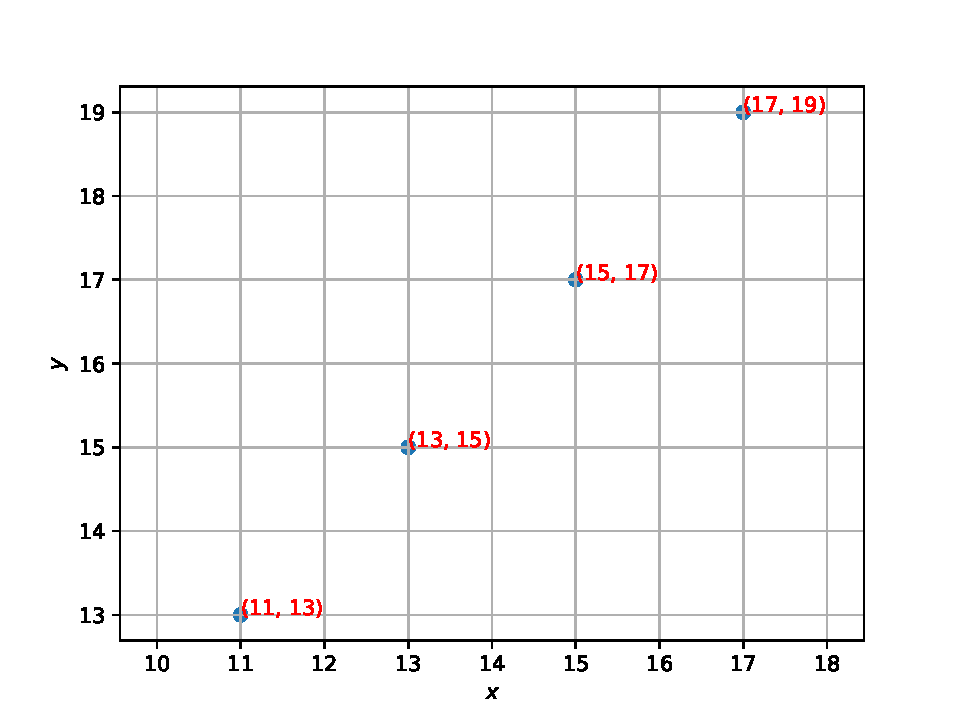
\includegraphics[width=\columnwidth]{./figs/lines/q15.pdf}
	\caption{Triangle of Q.3.11.5}
	\label{fig:qfifteen}	
	\end{figure}
	
	
\end{enumerate}

\section{\textbf{Question 4.1.5}}
\subsection{Problem}

\renewcommand{\theequation}{\theenumi}
\begin{enumerate}[label=\thesection.\arabic*.,ref=\thesection.\theenumi]
\numberwithin{equation}{enumi}
\item Find the area of the region in the first quadrant enclosed by the x-axis, the line $\myvec{1&-1}\vec{x}=0$ and the circle $\norm{\vec{x}}=1$.
The following python code computes the required area represented in Fig.\ref{fig:qseventeen}.
	\begin{lstlisting}
	./codes/circle/q17.py
	\end{lstlisting}
	
\solution
\begin{align}
\cos{\angle{BOA}} = \frac{\norm{\vec{OA}}^2 + \norm{\vec{OB}}^2 - \norm{\vec{AB}}^2}{2\norm{\vec{OA}}\norm{\vec{OB}}}
\\
\cos{\angle{BOA}} = \frac{1}{\sqrt{2}}
\\
\implies \angle{BOA} = 45\degree
\end{align}
 The required area is given by
\begin{align}
ar\brak{OACB} = \frac{\angle{BOA}}{360} \times \pi \times 1^2
\end{align}
\begin{comment}
\begin{align} 
ar\brak{OACB} = ar\brak{OAB} + ar\brak{ACB}\\
ar\brak{OACB} = \int\limits_{0}^{0.707} x dx + \int\limits_{0.707}^{1} \sqrt{1-x^2}dx
\end{align}
\end{comment}
which on computing, we obtain the required area as 0.3924
\begin{figure}[!ht]
	\centering
	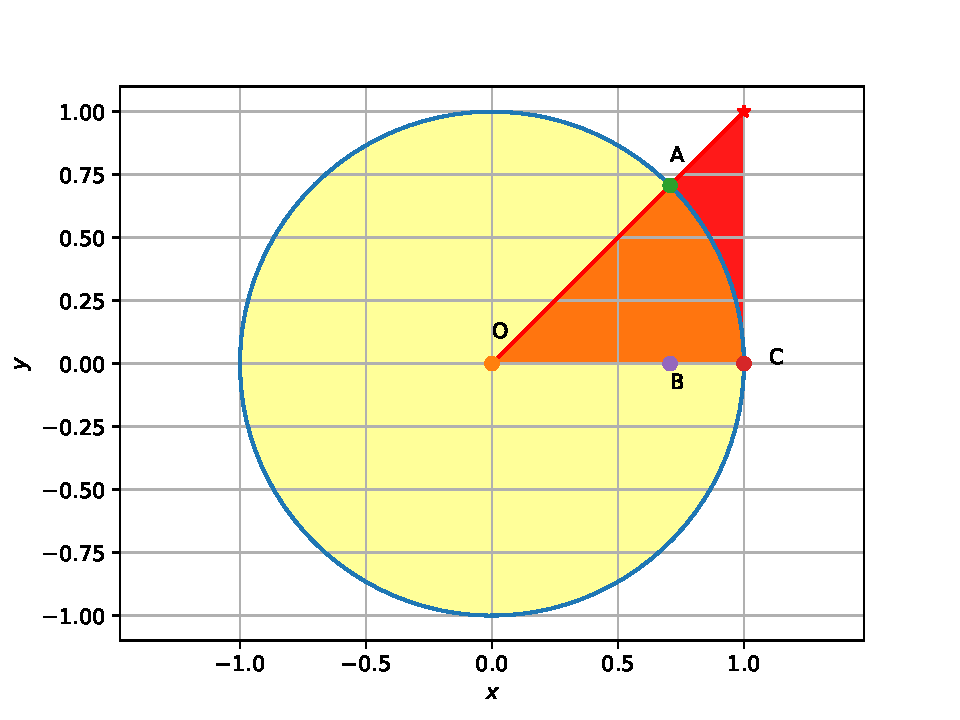
\includegraphics[width=\columnwidth]{./figs/circle/q17.pdf}
	\caption{Figure of Q.4.1.5}
	\label{fig:qseventeen}	
	\end{figure}
	
\end{enumerate}

\section{\textbf{Question 4.2.5}}
\subsection{Problem}

\renewcommand{\theequation}{\theenumi}
\begin{enumerate}[label=\thesection.\arabic*.,ref=\thesection.\theenumi]
\numberwithin{equation}{enumi}
\item Sketch circles with equation:
The following python codes generate the required circles :
	\begin{lstlisting}
	./codes/circle/q18abc.py
	./codes/circle/q18d.py
	\end{lstlisting}


\begin{enumerate}

\item \begin{multline} 
\vec{x^Tx} - \myvec{4\\8}\vec{x} -45 = 0\text{ represented in Fig:\ref{fig:qoeabc}}
\\
\text{Center is }\myvec{2\\4}\quad\text{Radius is }\sqrt{65}
\end{multline}

	\begin{figure}[!ht]
	\centering
	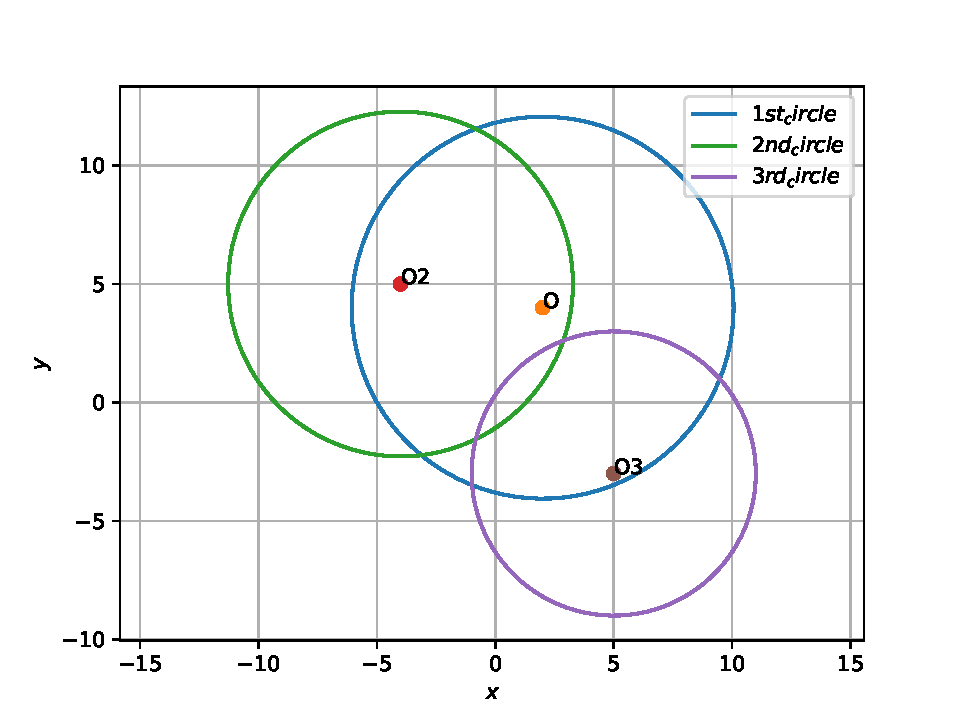
\includegraphics[width=\columnwidth]{./figs/circle/q18abc.pdf}
	\caption{Circle of Q.4.2.5}
	\label{fig:qoeabc}	
	\end{figure}

\item \begin{multline} 
\vec{x^Tx} - \myvec{8\\-10}\vec{x} - 12 = 0\text{ represented in Fig:\ref{fig:qoeabc}}
\\
\text{Center is }\myvec{-4\\5}\quad\text{Radius is }\sqrt{53}
\end{multline}


\item \begin{multline} 
\norm{x - \myvec{5\\-3}} = 36\text{ represented in Fig:\ref{fig:qoeabc}}
\\
\text{Center is }\myvec{5\\-3}\quad\text{Radius is }6
\end{multline}



\begin{comment}
	\begin{figure}[!ht]
	\centering
	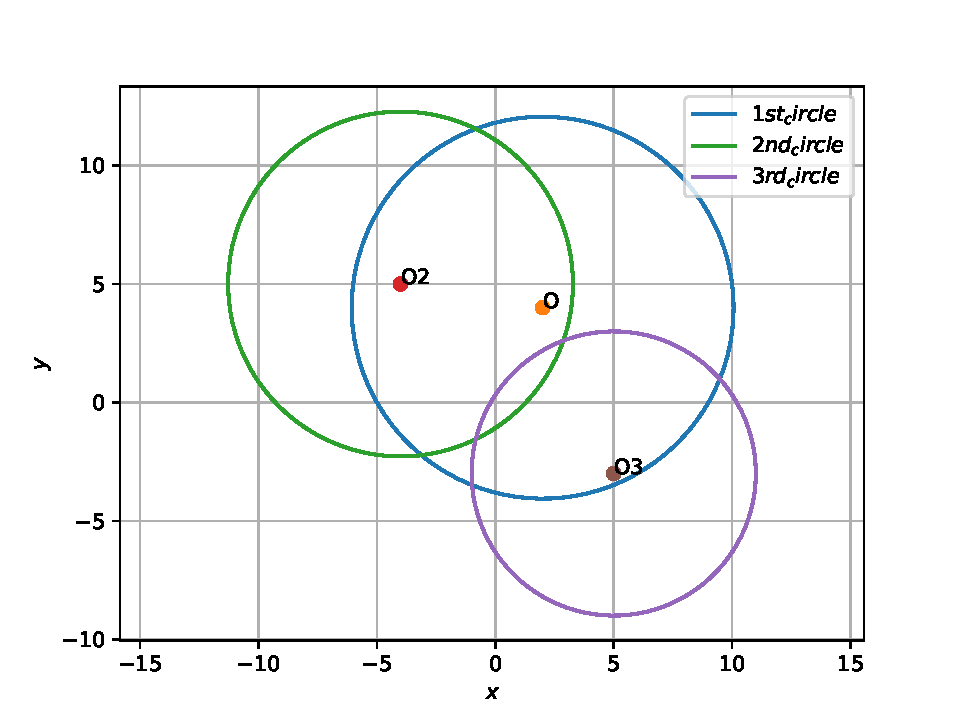
\includegraphics[width=\columnwidth]{./figs/circle/q18abc.pdf}
	\caption{Circle of Q.4.2.5}
	\label{fig:qoeb}	
	\end{figure}
\end{comment}
\begin{comment}
	\begin{figure}[!ht]
	\centering
	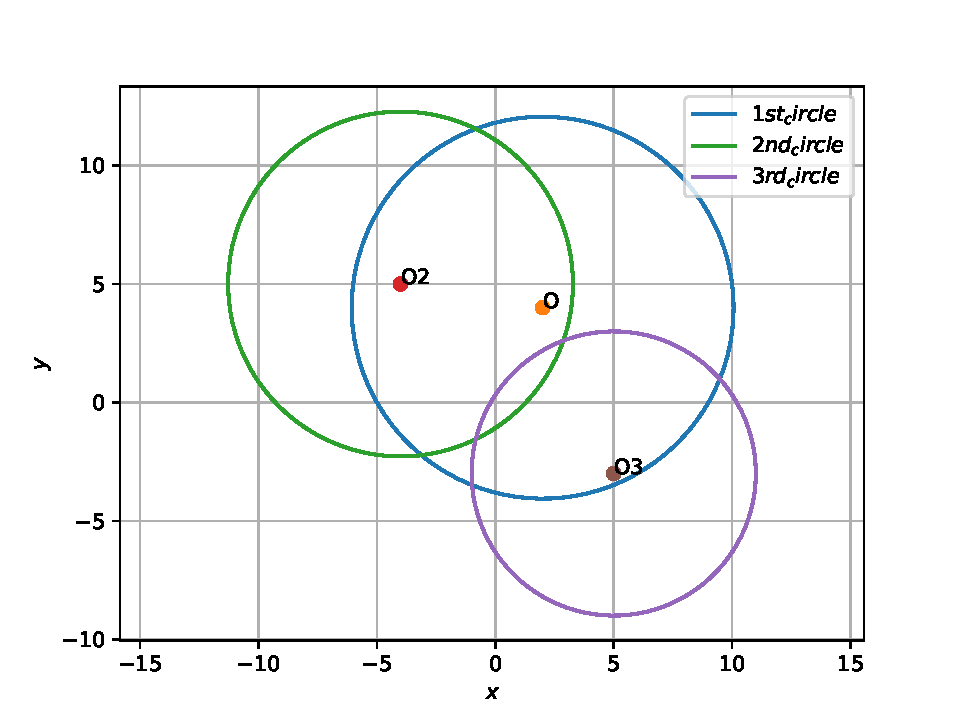
\includegraphics[width=\columnwidth]{./figs/circle/q18abc.pdf}
	\caption{Circle of Q.4.2.5}
	\label{fig:qoec}	
	\end{figure}
\end{comment}
\item \begin{multline} 
2\vec{x^Tx} - \myvec{1\\0}\vec{x} = 0\text{ represented in Fig:\ref{fig:qoed}}
\\
\text{Center is }\myvec{0.25\\0}\quad\text{Radius is }0.25
\end{multline}
	\begin{figure}[!ht]
	\centering
	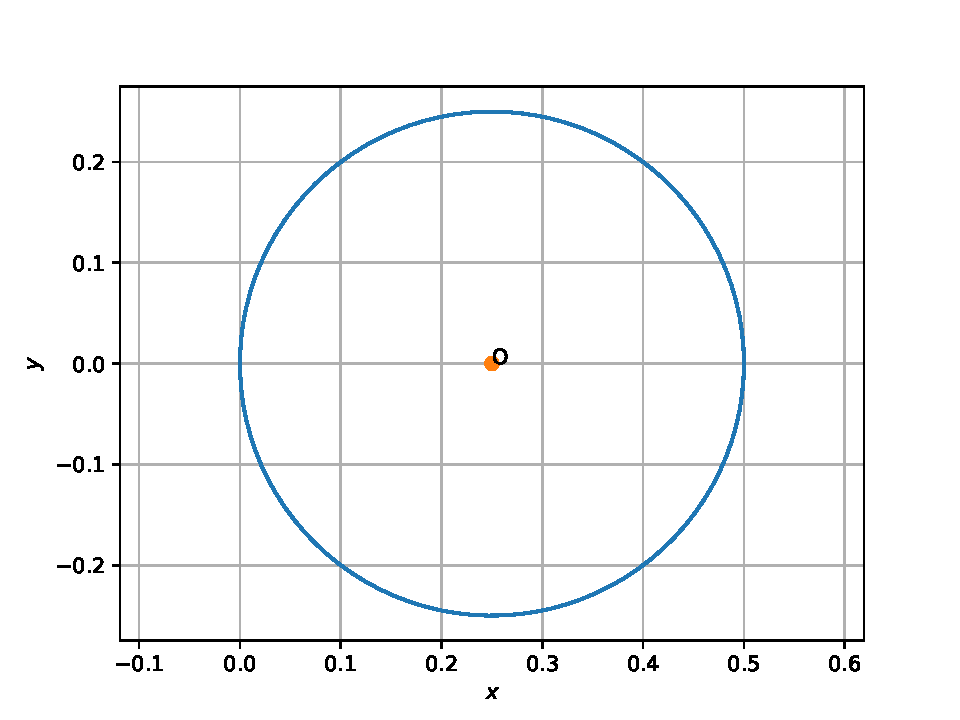
\includegraphics[width=\columnwidth]{./figs/circle/q18d.pdf}
	\caption{Circle of Q.4.2.5}
	\label{fig:qoed}	
	\end{figure}



\end{enumerate}
\end{enumerate}

\section{\textbf{Question 5.1.5}}
\subsection{Problem}

\renewcommand{\theequation}{\theenumi}
\begin{enumerate}[label=\thesection.\arabic*.,ref=\thesection.\theenumi]
\numberwithin{equation}{enumi}
	\item Find the roots of the quadratic equation $6x^2-x-2=0$.
	The following python code computes roots of the quadratic equation represented in Fig.\ref{fig:qnineteen}.
	\begin{lstlisting}
	./codes/conics/q19.py
	\end{lstlisting}
	
	\solution For a general polynomial equation of degree 2,
	\begin{multline}
	p\brak{x,y} \implies Ax^2 +Bxy + Cy^2 +Dx + Ey + F = 0
	\\
	\text{The vector form is}
	\\
	\vec{x}^T\myvec{A&\frac{B}{2}\\\frac{B}{2}&C}\vec{x}  + \myvec{D&E}\vec{x} + F = 0 \label{eq:theend}
	\end{multline}
	Here \begin{align}y = 6x^2-x-2 \quad \text{The vector form is}
	\\
	\vec{x}^T\myvec{6&0\\0&0}\vec{x}  + \myvec{-1&-1}\vec{x} -2 = 0
	\end{align}
	Thus, from \ref{eq:theend}
	\begin{align}
	y = 0 \quad \implies 6x^2-x-2 = 0
	\\
	\brak{x+\frac{1}{2}}\brak{x-\frac{2}{3}} = 0
	\\
	x = \frac{-1}{2},\frac{2}{3}
	\end{align}
\begin{comment}
	Using the quadratic formula,
	\begin{equation}
		x = \frac{-(-1) \pm \sqrt{(-1)^2 - 4(6)(-2)}}{2(6)}
	\end{equation}
	which on solving we get the roots as -0.5 and 0.666
\end{comment}
	\begin{figure}[!ht]
	\centering
	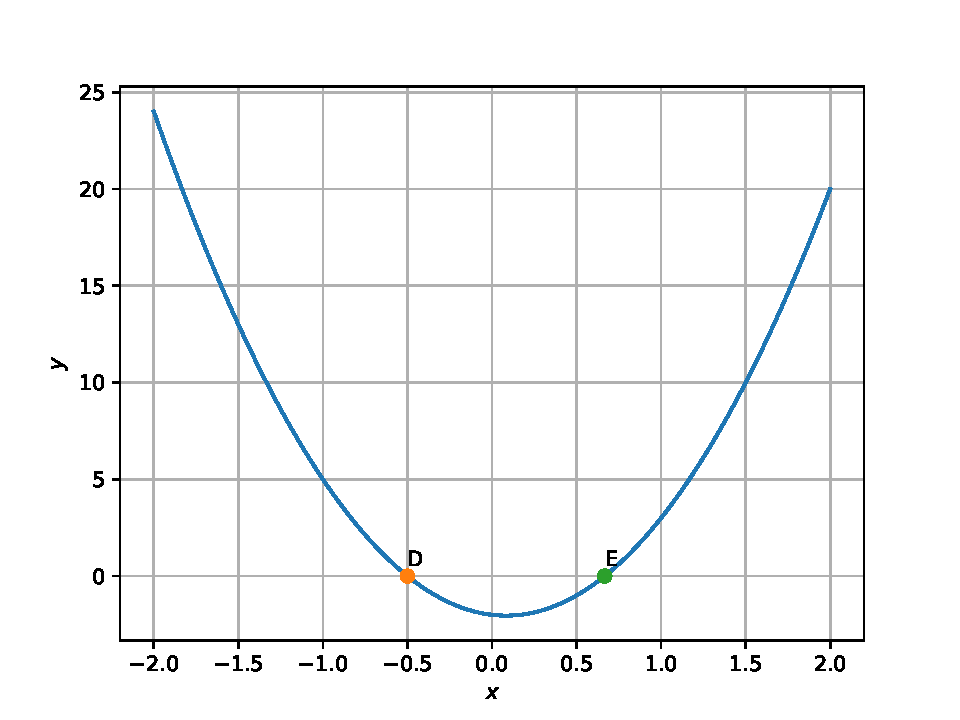
\includegraphics[width=\columnwidth]{./figs/conics/q19.pdf}
	\caption{Parabola of Q.5.1.5}
	\label{fig:qnineteen}	
	\end{figure}
	
	
\end{enumerate}

\section{\textbf{Question 5.2.5}}
\subsection{Problem}

\renewcommand{\theequation}{\theenumi}
\begin{enumerate}[label=\thesection.\arabic*.,ref=\thesection.\theenumi]
\numberwithin{equation}{enumi}

	\item Find a quadratic polynomial each with the given numbers as the sum and the product of its zeroes.
	\begin{enumerate}
	
		\item -1,$\frac{1}{4}$
		\\
		\solution For a general polynomial equation of degree 2,
	\begin{multline}
	p\brak{x,y} \implies Ax^2 +Bxy + Cy^2 +Dx + Ey + F = 0\\
	\text{The vector form is}\\
	\vec{x}^T\myvec{A&\frac{B}{2}\\\frac{B}{2}&C}\vec{x}  + \myvec{D&E}\vec{x} + F = 0 \label{eq:qtwenty}
	\end{multline}
Here, sum of zeroes = D = -1\\
Product of zeroes = F =$\frac{1}{4}$\\
Substituing the values in \ref{eq:qtwenty},\\
\begin{multline}
\vec{x}^T\myvec{1&0\\0&0}\vec{x}  + 
\myvec{1&-1}\vec{x} +\frac{1}{4} = 0\\
\end{multline}
\begin{align}
\implies y = x^2 + x + \frac{1}{4}
\end{align}
	
		
		\item 1,1
		\\
		\solution
Here, sum of zeroes = D = 1\\
Product of zeroes = F =1\\
Substituing the values in \ref{eq:qtwenty},\\
\begin{multline}
\vec{x}^T\myvec{1&0\\0&0}\vec{x}  + \myvec{-1&-1}\vec{x} +1 = 0
\end{multline}
\begin{align}
\implies y = x^2 - x + 1 
\end{align}
		
		\item 0,$\sqrt{5}$\\
		\solution
Here, sum of zeroes = D = 0\\
Product of zeroes = F =$\sqrt{5}$\\
Substituing the values in \ref{eq:qtwenty},\\
\begin{multline}
\vec{x}^T\myvec{1&0\\0&0}\vec{x}  + \myvec{0&-1}\vec{x} + \sqrt{5} = 0
\end{multline}
\begin{align}
\implies y = x^2 + \sqrt{5}  
\end{align}
		\item 4,1\\
		\solution 
Here, sum of zeroes = D = 4\\
Product of zeroes = F = 1\\
Substituing the values in \ref{eq:qtwenty},\\
\begin{multline}
\vec{x}^T\myvec{1&0\\0&0}\vec{x}  + \myvec{-4&-1}\vec{x} + 1 = 0
\end{multline}
\begin{align}
\implies y = x^2 - 4x + 1 
\end{align}


		\item $\frac{1}{4}$,$\frac{1}{4}$\\
\solution 
Here, sum of zeroes = D = $\frac{1}{4}$\\
Product of zeroes = F = $\frac{1}{4}$\\
Substituing the values in \ref{eq:qtwenty},\\

\begin{multline}
\vec{x}^T\myvec{1&0\\0&0}\vec{x}  + \myvec{-\frac{1}{4}&-1}\vec{x} + \frac{1}{4} = 0
\end{multline}
\begin{align}
\implies y = x^2 - \frac{1}{4}x + \frac{1}{4} 
\end{align}


		\item $\sqrt{2}$,$\frac{1}{3}$\\
\solution
Here, sum of zeroes = D = $\sqrt{2}$\\
Product of zeroes = F = $\frac{1}{3}$\\
Substituing the values in \ref{eq:qtwenty},\\
\begin{multline}
\vec{x}^T\myvec{1&0\\0&0}\vec{x}  + \myvec{-\sqrt{2}&-1}\vec{x} + \frac{1}{3} = 0
\end{multline}
\begin{align}
\implies y = x^2 - \sqrt{2}x + \frac{1}{3}
\end{align}
	\end{enumerate}
\end{enumerate}

\end{document}
